\documentclass[paper.tex]{subfiles}

\begin{document}

\section{Quandle Coloring of the (2,q)-torus knot}\label{sec:2ntorus}
\footnotetext{We will provide a means of deriving this in the next subsection: Matrix Representation}

\subsection{Recurrence Relation}

\begin{figure}[h]
  \centering
  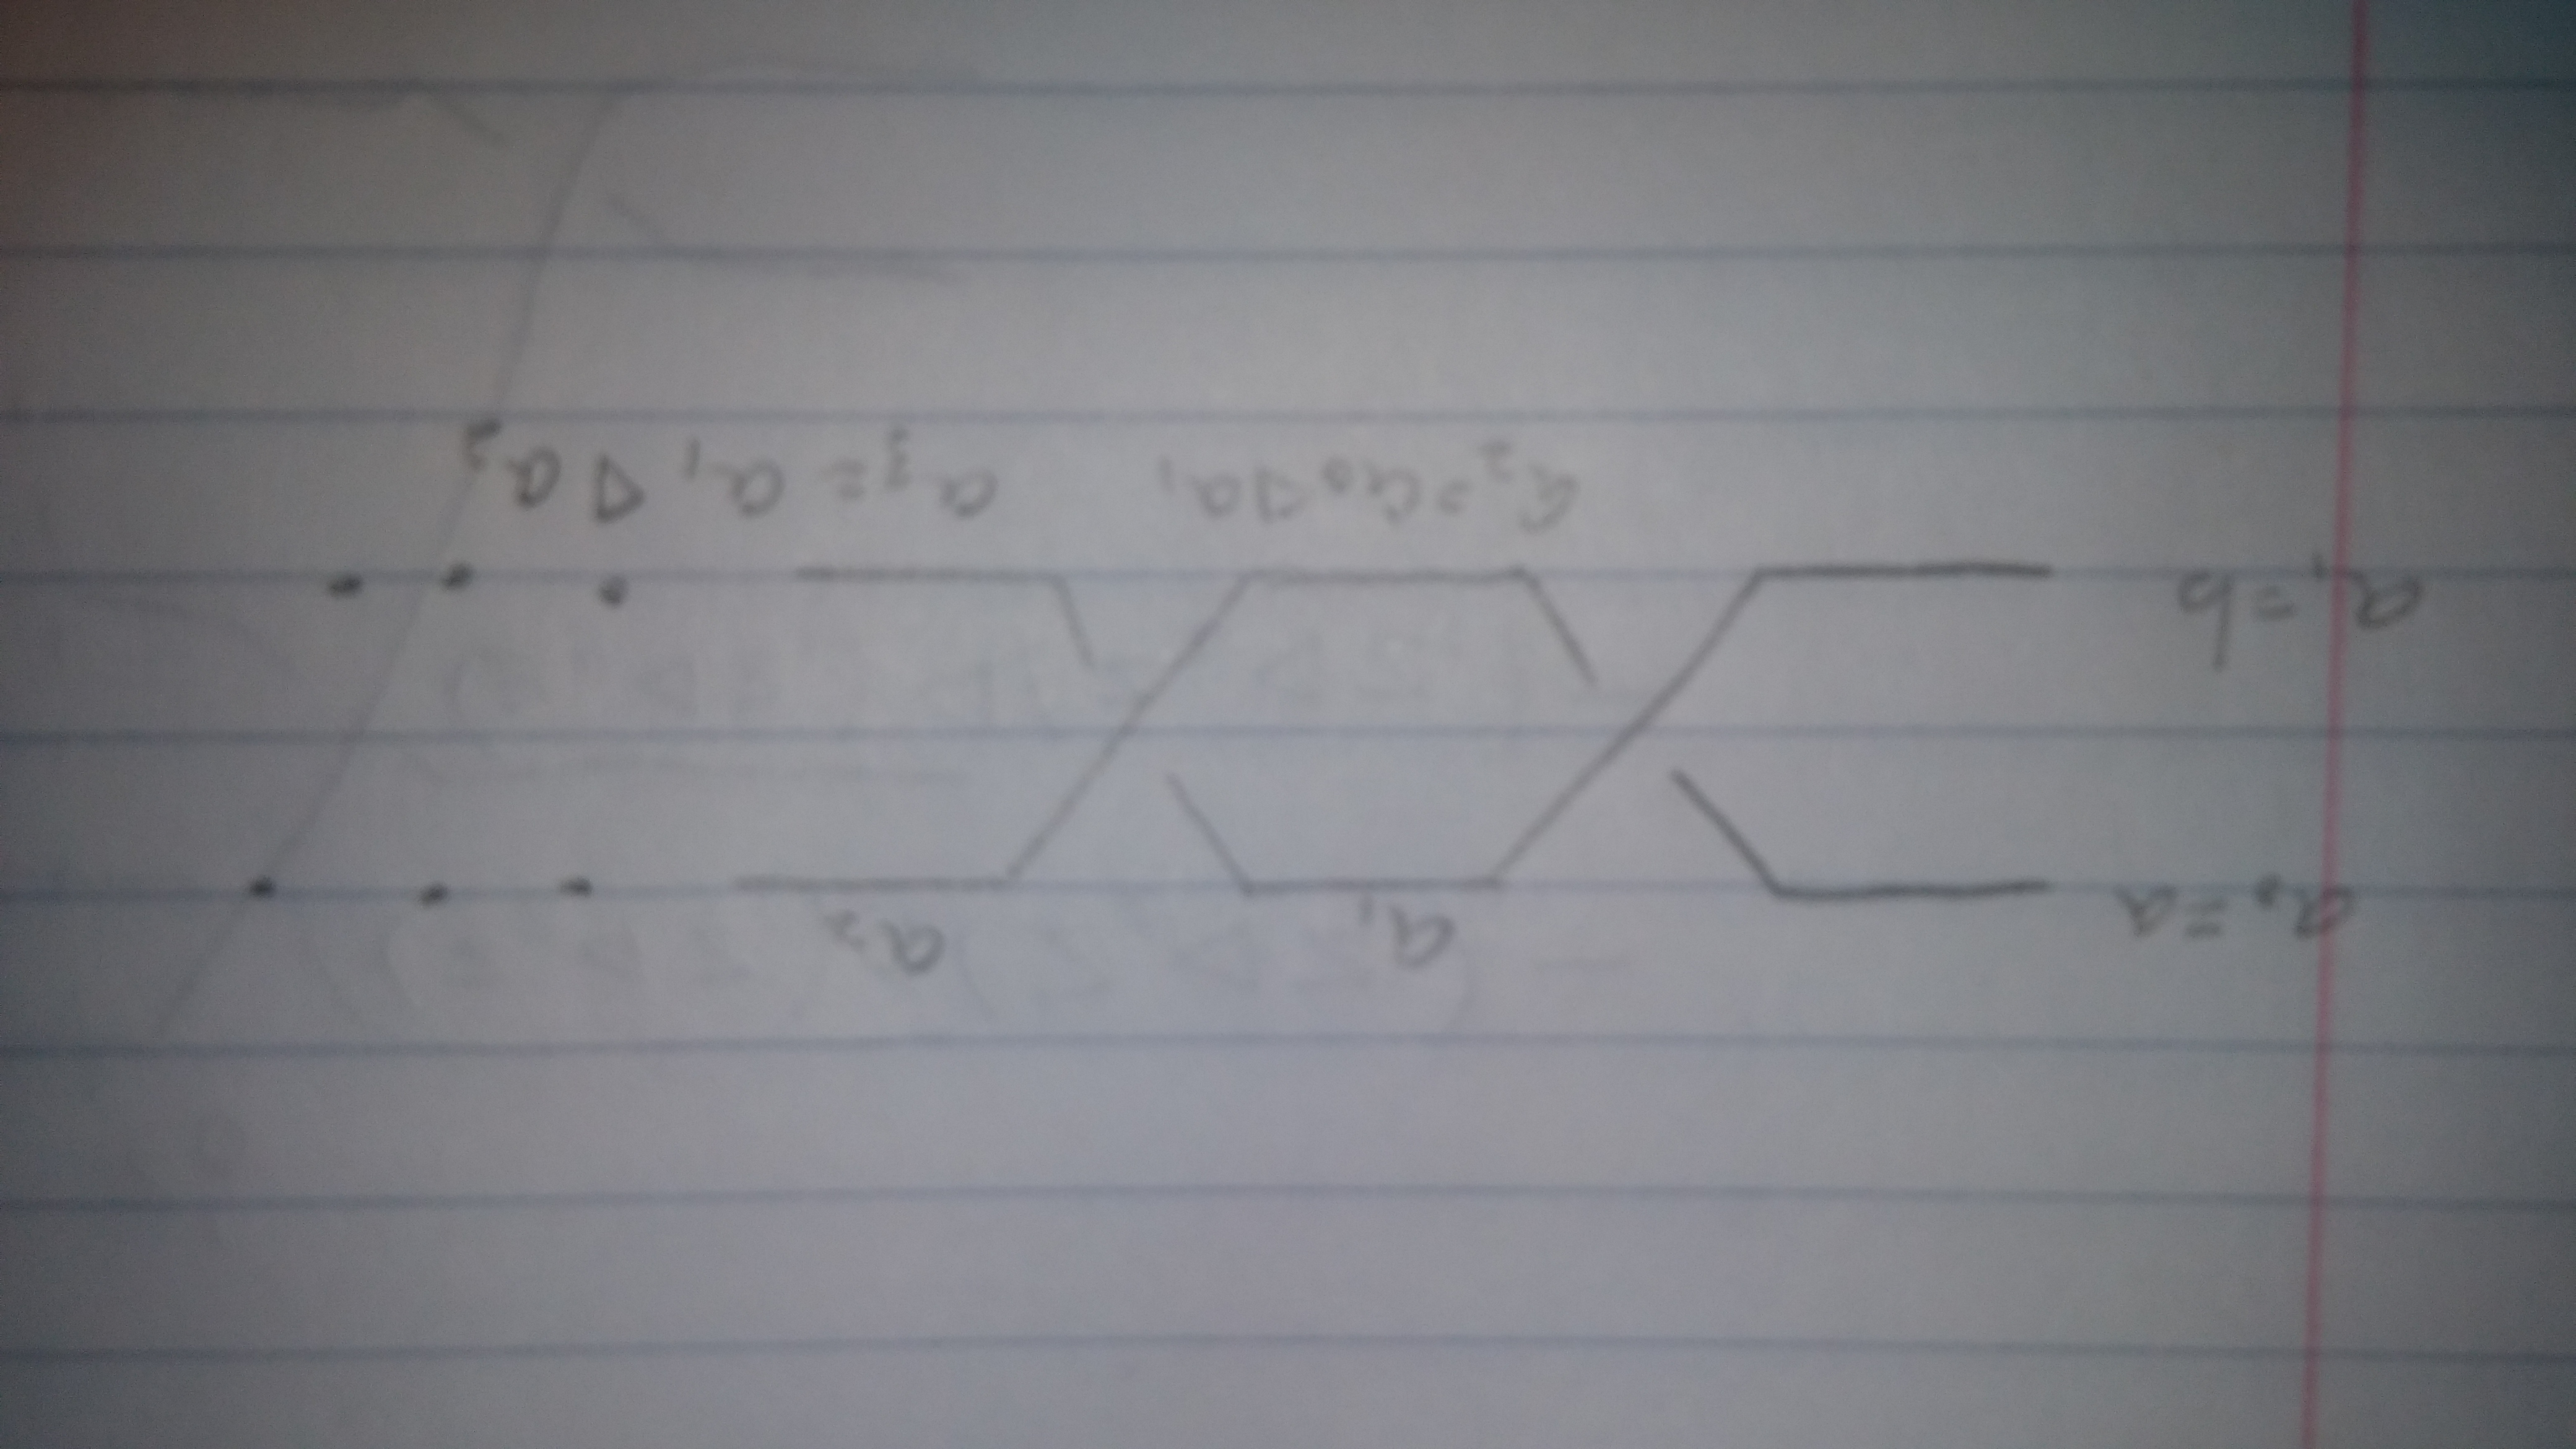
\includegraphics[width=0.8\textwidth]{2q}
  \caption{Visual representation of the recurrence relation $a_{n+2} = a_{n} \uc a_{n+1}$~\cite{Cusick}}\label{fig:2q}
\end{figure}

We first restrict ourselves to $(r,n)$-torus where $r = 2$. Secondly, we only concern ourselves with $\mathbb{Z}_p$ when $p > 2$ is prime.

In Figure ~\ref{fig:2q}, we can see that the $(2,n)$-torus knot satisfies the following recurrence relation:
\begin{align*}
	a_0 &= x \\
	a_1 &= y \\
	a_{n+2} &= a_{n} \uc a_{n+1} \\
\end{align*}

We can then substitute the Alexander quandle to conclude:

$$ a_{n+2} = qa_{n} + (1-q)b_{n+1} $$

Solving for\footnote{We will provide a proof of this in the next subsection: Matrix Representation}
 $a_n$ gives:

$$a_n = \frac{(-1)^nqx+q^nx+(-1)^{n+1}y+q^ny}{1+q}$$

To determine whether a knot is $\mathbb{Z}_{p,q}$ colorable we must solve for the system of equations so that $\forall x,y \in \mathbb{Z}_n$ the following holds:

\begin{align*}
	a_0 &\equiv a_{n}  & \mod{p} \\
	a_1 &\equiv a_{n+1} & \mod{p} \\
\end{align*}

We now know an explicit formula for $a_n$ so we may substitute it in accordingly:

\begin{align*}
	x &\equiv \frac{(-1)^nqx+q^nx+(-1)^{n+1}y+q^ny}{1+q} & \mod{p} \\
	y &\equiv \frac{(-1)^{n+1}qx+q^{n+1}x+(-1)^{n+2}y+q^{n+1}y}{1+q} & \mod{p} \\
\end{align*}

\subsection{Matrix Representation}

We consider an equivalent recurrence relation:

\begin{align*}
	a_{0} &= a_{p} \\
	a_{1} &= a_{p+1} \\
	x &= a_{p-2} + (1-q)a_{p-1} \\
	y &= a_{p-1} + (1-q)a_{p} \\
\end{align*}

To calculate $a_{p}$, we must find the matrix representation of
$$ a_{n} = (q)a_{n-2} + (1-q)a_{n-1} $$

\begin{align*}
\left[ \begin{array}{ccc}
a_{n} \\
a_{n-1} \\
\end{array} \right] 
&=
\left[ \begin{array}{ccc}
q & q-1 \\
0 & 1 \\
\end{array} \right]
\left[ \begin{array}{ccc}
 a_{n-2}\\
a_{n-1} \\
\end{array} \right] \\
\left[ \begin{array}{ccc}
a_{1} \\
a_{0} \\
\end{array} \right] 
&=
\left[ \begin{array}{ccc}
y \\
x \\
\end{array} \right] \\
\left[ \begin{array}{ccc}
a_{n} \\
a_{n-1} \\
\end{array} \right] 
&=
\left[ \begin{array}{ccc}
q-1 & q \\
1 & 0 \\
\end{array} \right] ^{n-1}
\left[ \begin{array}{ccc}
 a_{n-1}\\
a_{n-2} \\
\end{array} \right]
\end{align*}

Thus:

\begin{align*}
\left[ \begin{array}{ccc}
y \\
x \\
\end{array} \right] 
&=
\left[ \begin{array}{ccc}
a_{p+1} \\
a_{p} \\
\end{array} \right] \\
\left[ \begin{array}{ccc}
y \\
x \\
\end{array} \right] 
&=
\left[ \begin{array}{ccc}
q & q-1 \\
0 & 1 \\
\end{array} \right] ^{p}
\left[ \begin{array}{ccc}
y \\
x \\
\end{array} \right] \\
\left[ \begin{array}{ccc}
y \\
x \\
\end{array} \right] 
&=
A^{p}
\left[ \begin{array}{ccc}
y \\
x \\
\end{array} \right] \\
\end{align*}

\begin{align*}
A^{p} &= 
\left[ \begin{array}{ccc}
q-1 & q \\
1 & 0 \\
\end{array} \right] ^{p}
=
PD^{p}P^{-1} \\ 
A &= 
\left[ \begin{array}{ccc}
q-1 & q \\
1 & 0 \\
\end{array} \right]
=
PDP^{-1} \\ 
P &= 
\left[ \begin{array}{ccc}
-1 & q \\
1 & 1 \\
\end{array} \right] \\
P^{-1} &=
\left[ \begin{array}{ccc}
-(q+1)^{-1} & q(q+1)^{-1} \\
(q+1)^{-1} & (q+1)^{-1} \\
\end{array} \right] \\
D &= 
\left[ \begin{array}{ccc}
-1 & 0 \\
0 & q \\
\end{array} \right] \\ 
A^{p}
&=
\left[ \begin{array}{ccc}
-1 & q \\
1 & 1 \\
\end{array} \right]
\left[ \begin{array}{ccc}
-1 & 0 \\
0 & q \\
\end{array} \right] ^{p}
\left[ \begin{array}{ccc}
-(q+1)^{-1} & q(q+1)^{-1} \\
(q+1)^{-1} & (q+1)^{-1} \\
\end{array} \right] \\
A^{p}
&=
\left[ \begin{array}{ccc}
-1 & q \\
1 & 1 \\
\end{array} \right]
\left[ \begin{array}{ccc}
-1 & 0 \\
0 & q^{p} \\
\end{array} \right]
\left[ \begin{array}{ccc}
-(q+1)^{-1} & q(q+1)^{-1} \\
(q+1)^{-1} & (q+1)^{-1} \\
\end{array} \right] \\
A^{p} &=
\left[ \begin{array}{ccc}
\frac{q^{p+1} + (-1)^{p+1}}{q+1} & \frac{q^{p+1} + (-1)^{p}(q)}{q+1} \\
\frac{q^{p} + (-1)^{p+1}}{q+1} & \frac{q^{p} + (-1)^{p}(q)}{q+1} \\
\end{array} \right] \\
\left[ \begin{array}{ccc}
y \\
x \\
\end{array} \right]&=
A^{p}
\left[ \begin{array}{ccc}
y \\
x \\
\end{array} \right] \\
\left[ \begin{array}{ccc}
y \\
x \\
\end{array} \right]&=
\left[ \begin{array}{ccc}
y \frac{q^{p+1} + (-1)^{p+1}}{q+1} + x \frac{q^{p+1} + (-1)^{p}(q)}{q+1} \\
y \frac{q^{p} + (-1)^{p+1}}{q+1} + x \frac{q^{p} + (-1)^{p}(q)}{q+1} \\
\end{array} \right] \\
\end{align*}

Which confirms

$$x = \frac{(-1)^nqx+q^nx+(-1)^{n+1}y+q^ny}{1+q} \mod p $$

A $(2,n)$-torus knot $\gcd(2,n) = 1$, therefore, $n$ must be odd. We can then simplify the congruences to the following:

\begin{align*}
	x &\equiv \frac{-qx+q^nx+y+q^ny}{1+q} & \mod{p} \\
	y &\equiv \frac{qx+q^{n+1}x-y+q^{n+1}y}{1+q} & \mod{p} \\
\end{align*}

From this point, we can arrive upon the $Z_{p,q}$ quandle colorings of any $T(2, p)$ torus knot. Find all $q$ satisfying the equivalence relation above $\forall x,y \in \mathbb{Z}_n$

\section{Quandle Coloring of the (3,q)-torus knot}\label{sec:3ntorus}
We first restricted ourselves to $T(2,p)$-torus knots. Conveniently, we were able to derive an easily diagonalizable recurrence relation matrix, $A$. Now, we are going to try and extend this $Z_{p,q}$ quandle coloring to all $T(p,3)$ knots.

Remember, the $(2,n)$-torus knot satisfies the following recurrence relation:
\begin{align*}
	a_0 &= x \\
	a_1 &= y \\
	a_{n+2} &= a_{n} \uc a_{n+1} \\
\end{align*}

Using the braid word of a $T(3,p)$-torus knot, the quandle coloring satisfies two recurrence relations that depending on the parity of $n$:
\begin{align*}
	a_0 &= x \\
	a_1 &= y \\
	a_2 &= z \\
\end{align*}
\begin{align*}
	a_{n} &= a_{n-3} \triangleleft a_{n-2} \\
	a_{n-1} &= a_{n-4} \triangleleft a_{n-2} \\
\end{align*}

Here, there recurrence relation for odd and even values of $n$ are not equivalent. Thus, the recurrence relation matrix, $A$, for the $T(3, p)$ Alexander Quandle has two forms. $A_{0}$ for calculating $a_{n}$ when $n \equiv 0 \mod 2$. $A_{1}$ is for calculating $a_{n}$ when $n \equiv 1 \mod 2$:

\[ A_{0} =
\left[ \begin{array}{ccc}
q-1 & q & 0 \\
q-1 & 0 & q \\
1 & 0 & 0 \\
\end{array} \right]
\]
\[ A_{1} =
\left[ \begin{array}{ccc}
q-1 & 0 & q \\
q-1 & q & 0 \\
1 & 0 & 0 \\
\end{array} \right]
\]

If $n \equiv 0 \mod 2$:

\[
\left[ \begin{array}{ccc}
a_{n} \\
a_{n-1} \\
a_{n-2} \\
\end{array} \right]
=
\left[ \begin{array}{ccc}
q-1 & q & 0 \\
q-1 & 0 & q \\
1 & 0 & 0 \\
\end{array} \right]
\left[ \begin{array}{ccc}
a_{n-2} \\
a_{n-3} \\
a_{n-4} \\
\end{array} \right]
\]

If $n \equiv 1 \mod 2$:

\[
\left[ \begin{array}{ccc}
a_{n} \\
a_{n-1} \\
a_{n-2} \\
\end{array} \right]
=
\left[ \begin{array}{ccc}
q-1 & 0 & q \\
q-1 & q & 0 \\
1 & 0 & 0 \\
\end{array} \right]
\left[ \begin{array}{ccc}
a_{n-2} \\
a_{n-3} \\
a_{n-4} \\
\end{array} \right]
\]


We can start calculating successive entries in the sequence {$a_{n}$}:

\[
\left[ \begin{array}{ccc}
a_{3} \\
a_{2} \\
a_{1} \\
\end{array} \right]
=
\left[ \begin{array}{ccc}
q-1 & 0 & q \\
q-1 & q & 0 \\
1 & 0 & 0 \\
\end{array} \right]
\left[ \begin{array}{ccc}
z \\
y \\
x \\
\end{array} \right]
\]

\[
\left[ \begin{array}{ccc}
a_{4} \\
a_{3} \\
a_{2} \\
\end{array} \right]
=
\left[ \begin{array}{ccc}
q-1 & q & 0 \\
q-1 & 0 & q \\
1 & 0 & 0 \\
\end{array} \right]
\left[ \begin{array}{ccc}
q-1 & 0 & q \\
q-1 & q & 0 \\
1 & 0 & 0 \\
\end{array} \right]
\left[ \begin{array}{ccc}
z \\
y \\
x \\
\end{array} \right]
\]

\[
\left[ \begin{array}{ccc}
a_{n} \\
a_{n-1} \\
a_{n-2} \\
\end{array} \right]
=
\left[ \begin{array}{ccc}
q-1 & q & 0 \\
q-1 & 0 & q \\
1 & 0 & 0 \\
\end{array} \right] ^{n//2}
\left[ \begin{array}{ccc}
q-1 & 0 & q \\
q-1 & q & 0 \\
1 & 0 & 0 \\
\end{array} \right] ^{(n//2) + n\%2)}
\left[ \begin{array}{ccc}
z \\
y \\
x \\
\end{array} \right]
\]

\[
\left[ \begin{array}{ccc}
a_{n} \\
a_{n-1} \\
a_{n-2} \\
\end{array} \right]
=
\left[ \begin{array}{ccc}
q-1 & 0 & q \\
q-1 & q & 0 \\
1 & 0 & 0 \\
\end{array} \right] ^{n\%p}
\left[ \begin{array}{ccc}
(q-1)^{2} + q(q-1) & q^{2} & (q-1)q \\
(q-1)^{2} + q & 0 & (q-1)q \\
q-1 & 0 & q \\
\end{array} \right] ^{n//2}
\left[ \begin{array}{ccc}
z \\
y \\
x \\
\end{array} \right]
\]

Replicating the calculations of the $T(p,2)$ Alexander quandle equivalence relations, you can find the following equivalence relations:

\begin{align*}
	x \equiv P(x,y,z,q) & \mod{p} \\
	y \equiv P(x,y,z,q) & \mod{p} \\
	z \equiv P(x,y,z,q) & \mod{p} \\
\end{align*}

Given the complexity of the diagonal of $A^{p}$, we were unable to find a simplified form for

\[ A^{n}
=
\left[ \begin{array}{ccc}
q-1 & 0 & q \\
q-1 & q & 0 \\
1 & 0 & 0 \\
\end{array} \right] ^{n\%2}
\left[ \begin{array}{ccc}
(q-1)^{2} + q(q-1) & q^{2} & (q-1)q \\
(q-1)^{2} + q & 0 & (q-1)q \\
q-1 & 0 & q \\
\end{array} \right] ^{n//2}
\]

We suspect there are alternative or brute force methods available to solve the $T(p,3)$ Alexander quandle equivalence relations.  We have not calculated the explicit solution in terms of $q$ for this equivalence set due to computational capacity. Additional endeavors in efficient computing or decomposition of $A^{n}$ are needed to find a timely solution to the equivalence set for the $T(p,3)$ Alexander quandle representations.

%% \section{Conclusions: Quandle Coloring of the T(p,q)-torus knot}\label{sec:pntorus}
%% Although further calculations can be done to solve for $q$ in
%% \begin{align*}
%% 	x \equiv P(x,y,z,q) & \mod{p} \\
%% 	y \equiv P(x,y,z,q) & \mod{p} \\
%% 	z \equiv P(x,y,z,q) & \mod{p} \\
%% \end{align*}
%% we were able to define a process for finding the $Z_{p,q}$ Quandle Colorings of T(p, 3) and T(p,2) torus knots. By (1) finding the recurrence relation for quandle labeling of a T(p,q) torus knot, (2) representing the recurrence relation in terms of the alexander quandle, (3) constructiing a recurrence relation matrix,  (4) setting the quandle labeling equivalence relations ($a_{0} \equiv P(a_{0},...,a_{p},q) \mod{p}$) , and (5) solving for $q$ across $\forall x,y \in \mathbb{Z}_n$, we have defined a reasonable process for finding the $Z_{p,q}$ Quandle Colorings of $T(p,q)$ torus knots.

\section{A quandle relation for $T(p,q)$ knots}

In this section we derive a recurrence relation that a quandle coloring $T(p,q)$ must satisfy. We take advantage that every $T(p,q)$ knot has the very simple braid diagram representation $(B_p)^q$ (see Figure~\ref{fig:bp}). First,
we set some notation, adopting that of Figure~\ref{fig:braid_notation}. For a $(B_p)^q$ braid diagram, we call the strands, starting from the far left of the first $B_p$ $z^0_1, z^0_2, \ldots, z^0_p$ from top to bottom.
The right strands of the first copy of $B_p$, or equivalently, the left strands of the second copy of$B_p$ we notate analogously, changing the superscript to $1$. For instance, the right most strands in the diagram are called $z^{q - 1}_i$.

Additionally, we adopt $O_i$ as notation for the overcrossing strand in the $i - 1$th copy of $B_p$. The first overcrossing is called $O_0$.

\begin{figure}[h]
  \centering
  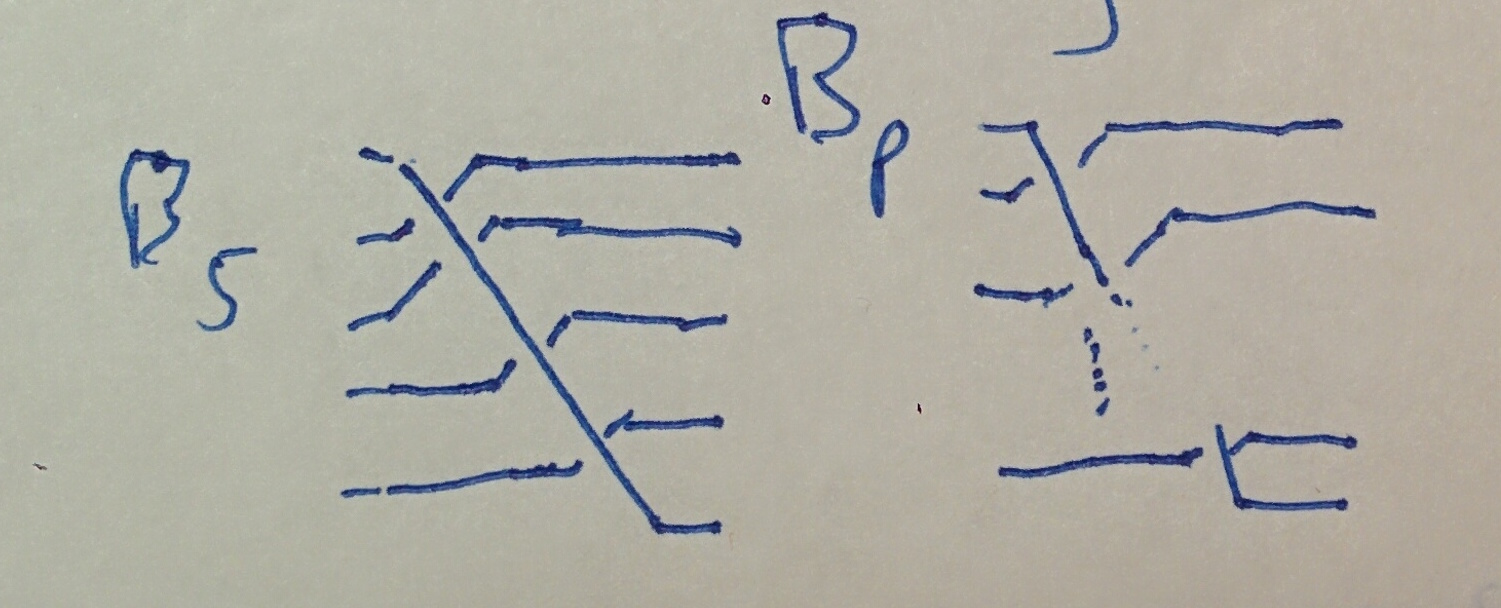
\includegraphics[width=0.8\textwidth]{b5}
  \caption{On the left, the braid $B_5$. On the right, $B_p$}\label{fig:bp}
\end{figure}

\begin{figure}[h]
   \centering
   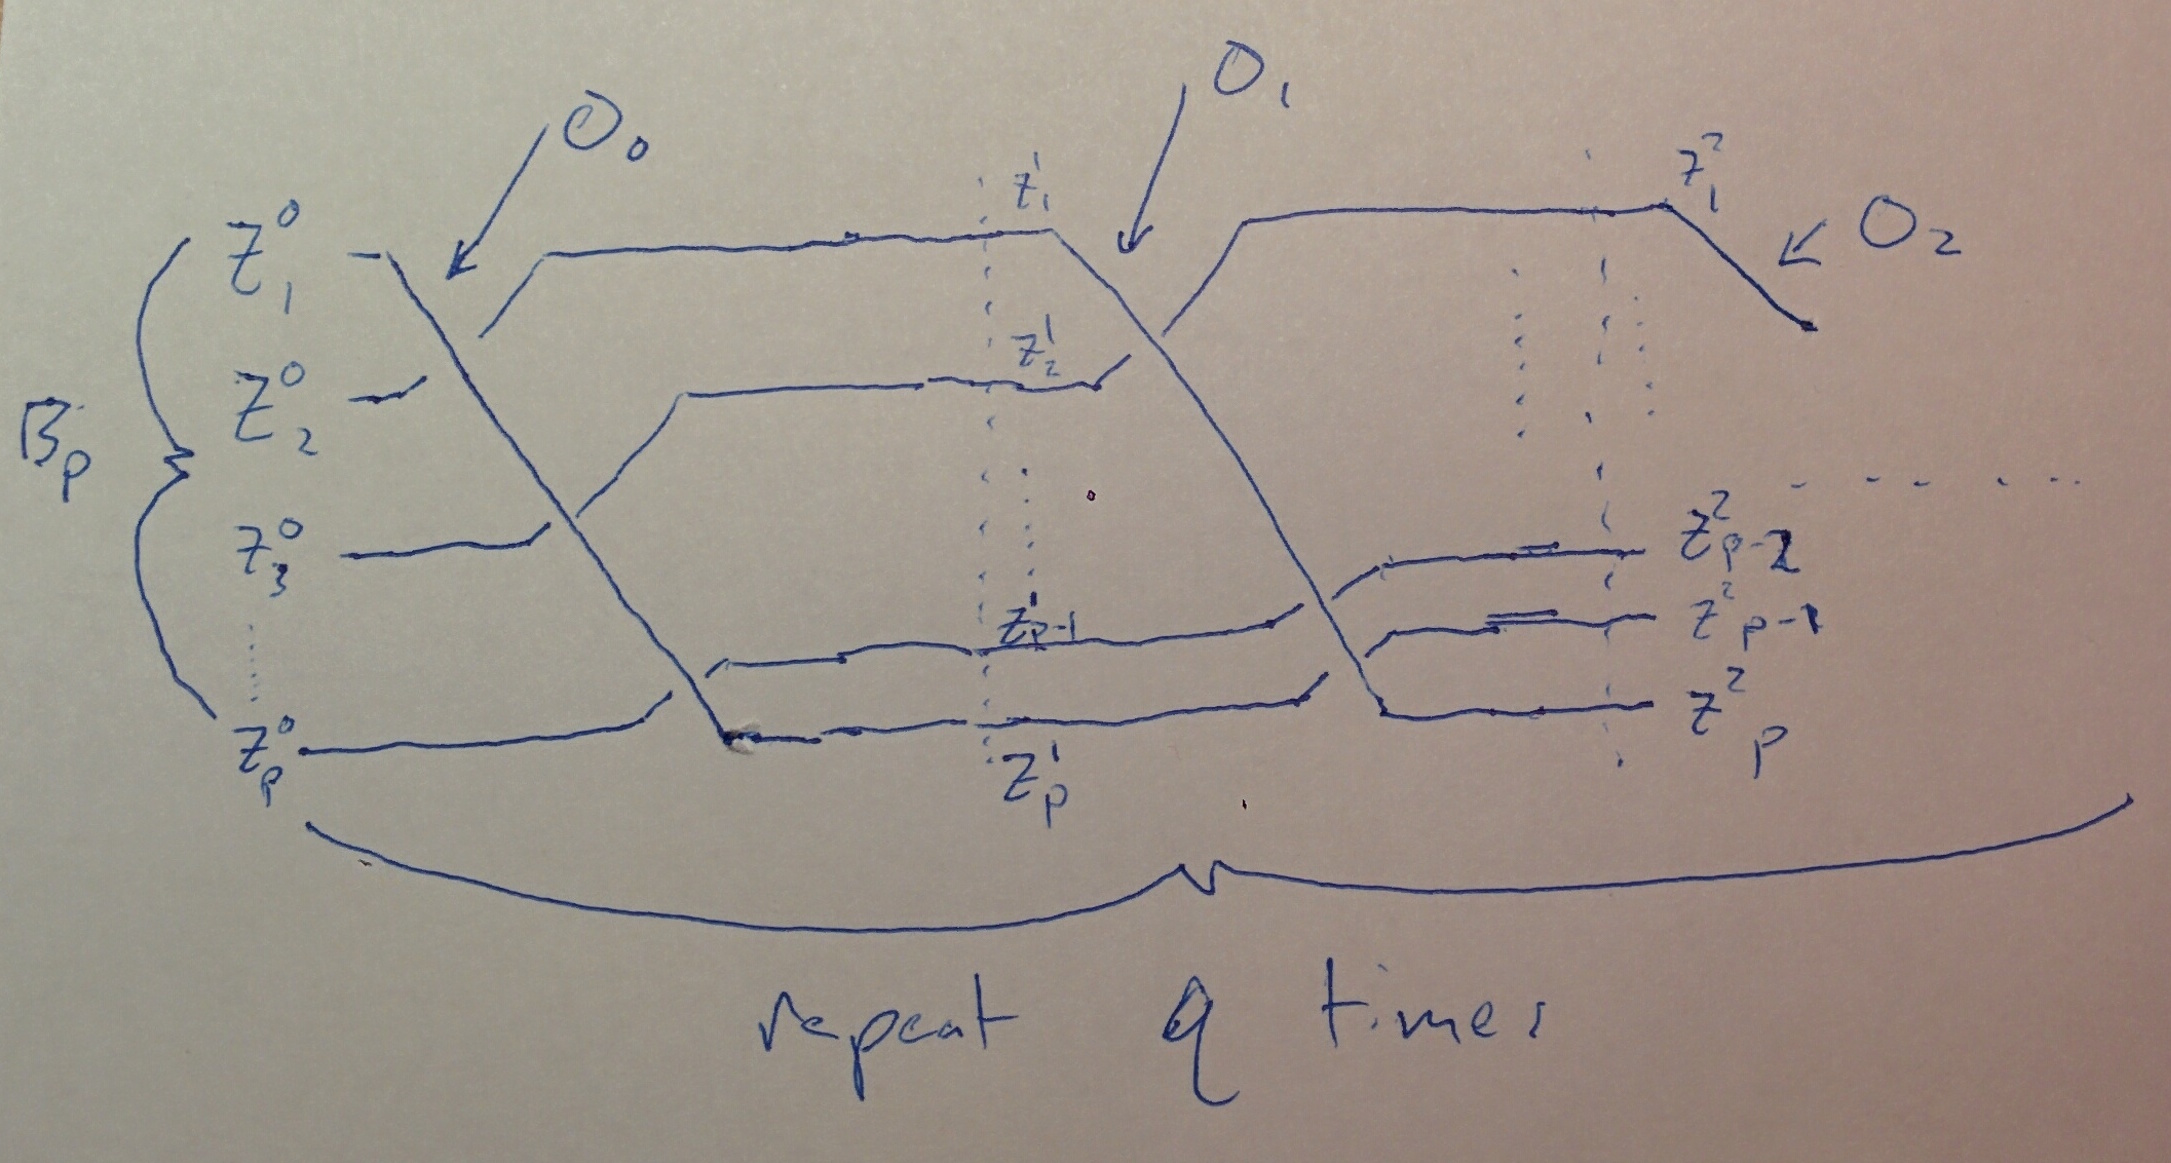
\includegraphics[width=0.8\textwidth]{braid_notation}
   \caption{The notation we adopt for braid diagrams.}\label{fig:braid_notation}
\end{figure}

With this setup, we easily derive the following recurrence relation

\begin{equation}
   \label{eq:pq_recurrence}
   z^{n+1}_l = \left\{
   \begin{matrix}
        z^n_{l+1} \uc O_n &\text{ if } l < p \\
        z^n_1 &\text{ if } l = p
   \end{matrix}
   \right.
\end{equation}

Furthermore it is easily seen that

\begin{equation}
   O_n = (\ldots((z_n \uc O_1) \uc O_2) \ldots ) \uc O_{n-1}
\end{equation}

Through successive application of the third quandle axiom (Equation~\ref{eq:ax3}), or alternatively, by playing with the knot diagram\footnote{Since quandles by construction satisfy the Redeimeister moves, you can do algebra
        on quandle colorings visually by playing with the knot diagram! Cool!} this can be seen to simplify into the possibly more transparent form

\begin{equation}
   O_n = (z_n \uc O_1) \uc (O_2 \uc O_{n -1}) \uc \ldots \uc (O_{n - 2} \uc O_{n - 1})
\end{equation}

Despite our best efforts, these relations resisted further simplification. Where we more skilled with Mathematica or had more time we would have substituted the $Z_{n,q}$ undercrossing operation into these relations
     and attempted to fully solve (by setting $z^q_{i} = z^0_{i}$) and simplify the generalized equivalence relation given in Equation~\ref{eq:bp_recurrence}. As it stands, this relation gives a prescription for
     determining if $T(r,k)$ is $\Z_{n,q}$ colorable, and for counting colorings. It shouldn't be more than a day's effort to use this relation to write such a program.

However, in order to exercise our general quandle relation, we used it to compute another relation (over $\Z_n$) for $T(2, k)$ knots. We omit the calculation, as it is fairly straightforward. The relation is, for fixed $p$
      and $q$ a unit $\Z_n$

\begin{align}
    z_l &= q^2 z_{l + 2} + q(1 - q) z_2 + (1 - q) z_1 \text{ for } l < p -1\\
    z_{p - 1} &= (1 - q + q^2) z_1 + (1 + q - q^2) z_2 \\
    z_p  &= q z_2 + (1 - q) z_2
\end{align}

\section{Further Questions}\label{fqs}

\begin{enumerate}
\item Consider what happens to $Z_{p,q}$ when $p$ is not prime.
\end{enumerate}


\end{document}
